\subsubsection{pr06}
\label{subsubsec:pr06}
The obtained results were the following:
{
\renewcommand{\arraystretch}{2}
\begin{longtable}[h]{| c | c | c | c | c |}
    \hline
    \textbf{Failures} & \multicolumn{3}{c}{Time limit} & \\
    \hline
    \textbf{Search strategy} & \textbf{\textit{30 sec}} & \textbf{\textit{1 min}} & \textbf{\textit{2 min}} & \textbf{\textit{5 min}} \\
    \hline
    \endhead
    default search                                         & 145 &  145 &  6.850 &  13.557 \\
    \hline
    domWdeg, random                                        &  74 &   74 &  6.779 &  13.486 \\
    \hline
    domWdeg, random, Luby restart L=250                    &  92 &   92 &   92 &    2.199 \\
    \hline
    \textit{domWdeg, random, Luby restart L=250, LNS 85\%} &  92 &   92 &   92 &      92 \\
    \hline
    domWdeg, random, Luby restart L=250, LNS 15\%          &  92 &   92 &   92 &    4.475 \\
    \hline
    first fail, min                                        &  16 &   16 & 6.721 &   13.430 \\
    \hline
\end{longtable}
}
\begin{figure}[H]
    \centering
    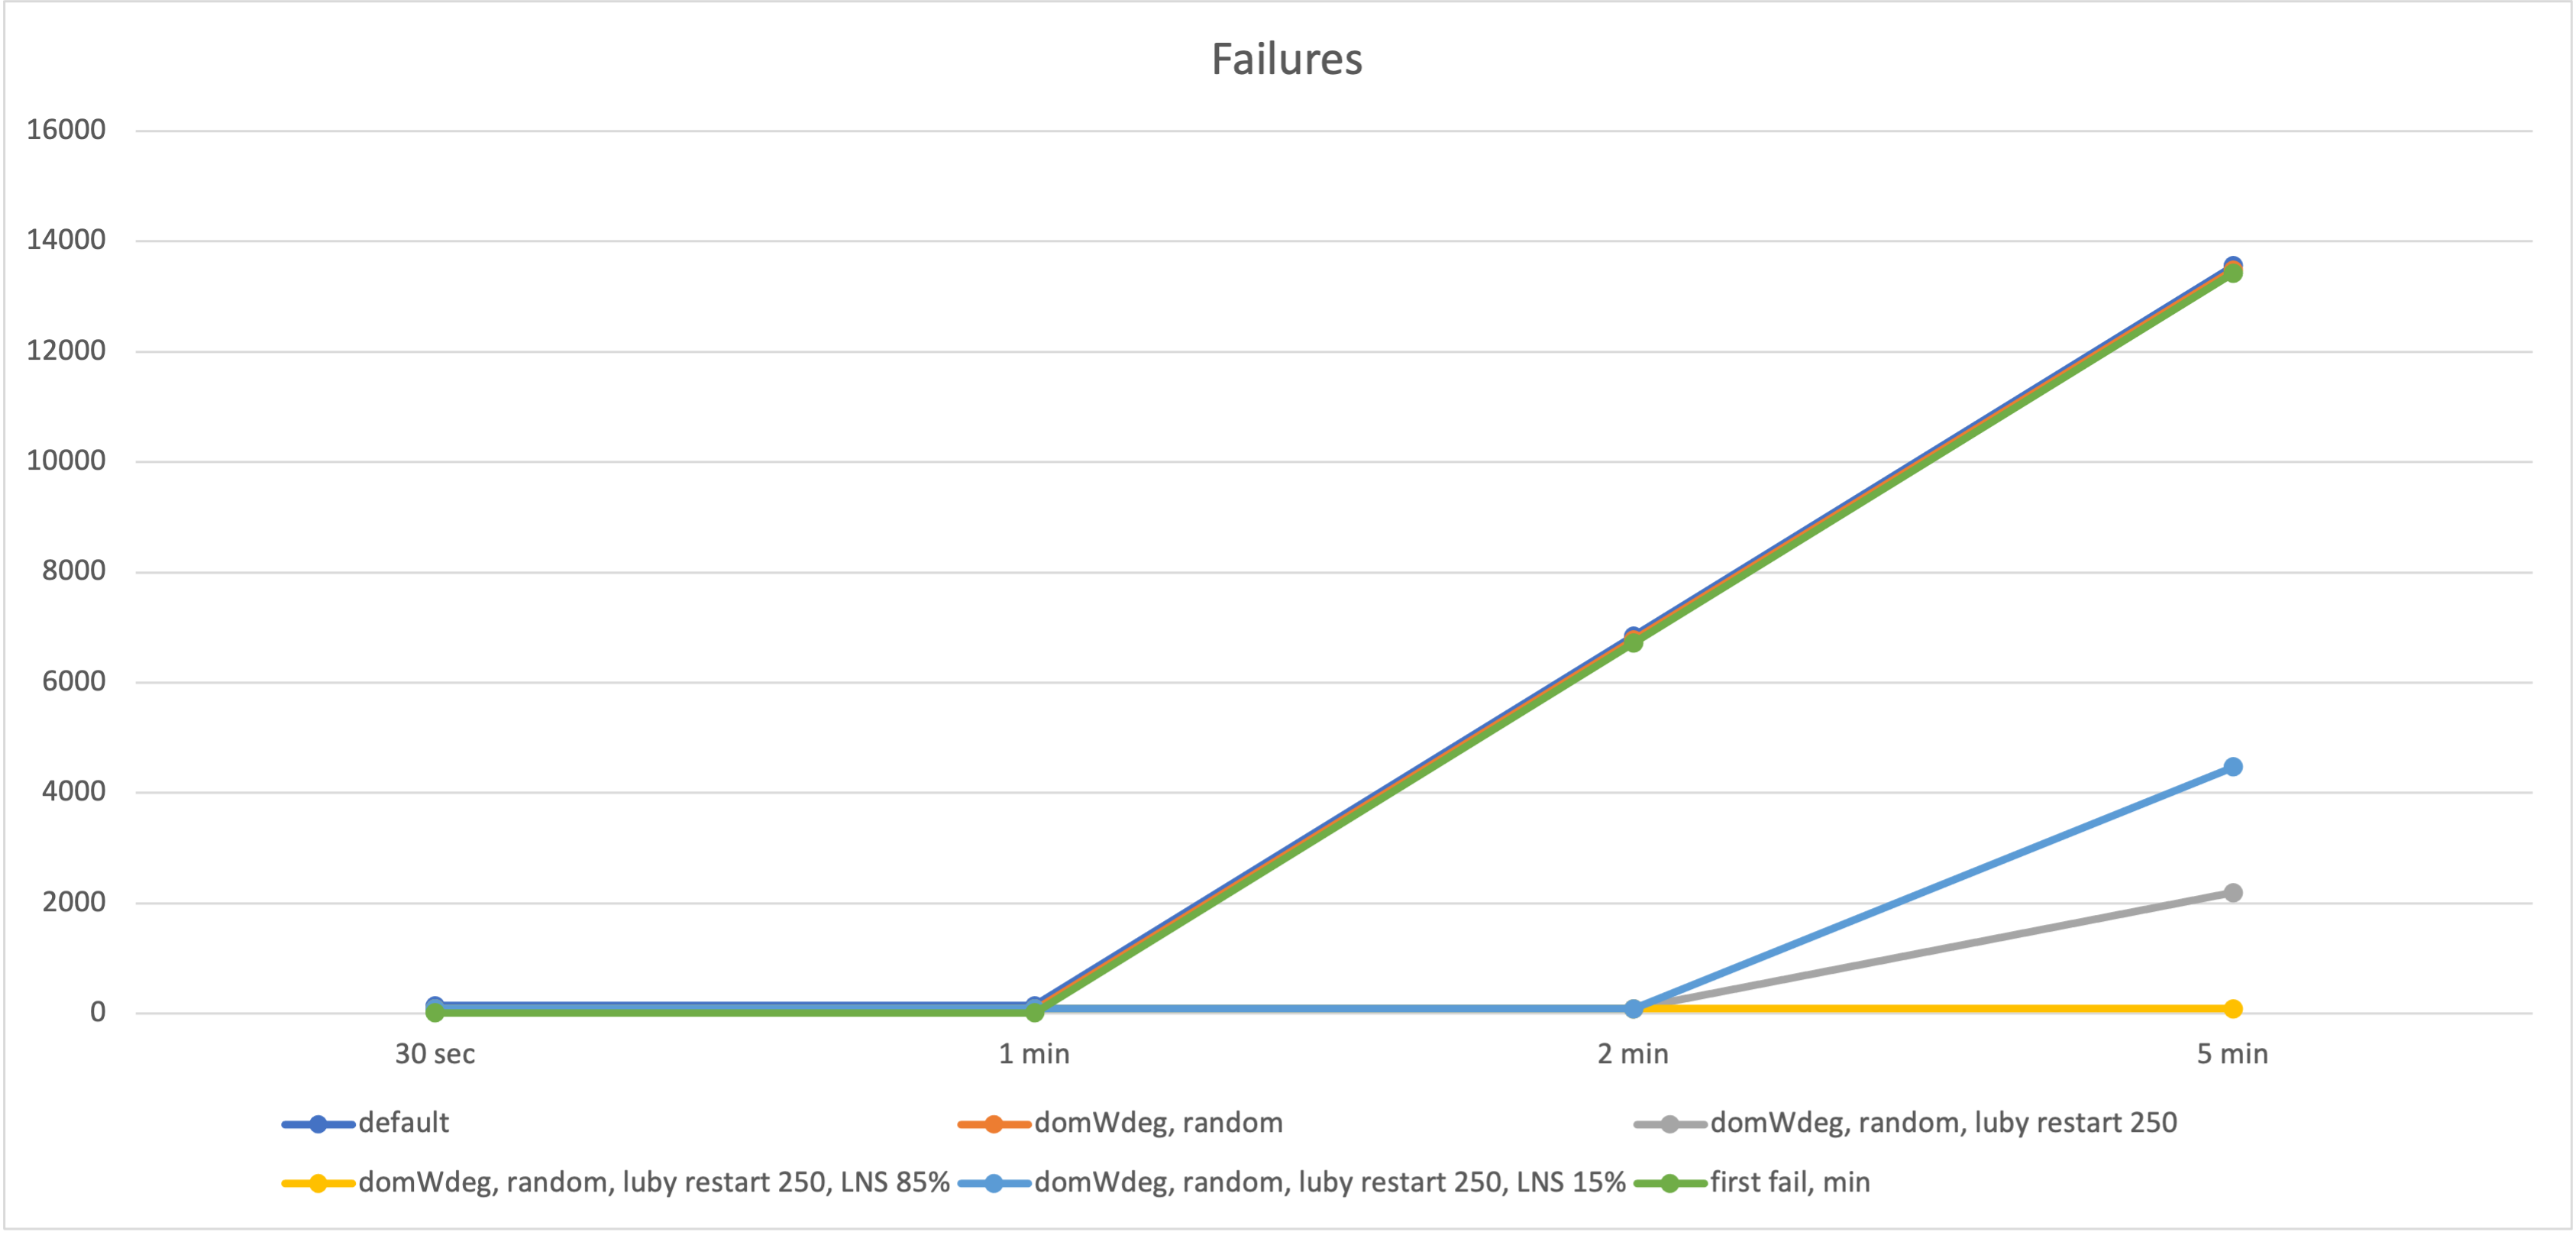
\includegraphics[width=0.8\columnwidth]{../graphs/pr06-failures.png}
    \caption{Failures graph for \textbf{pr06}.}
\end{figure}

{
\renewcommand{\arraystretch}{2}
\begin{longtable}[h]{| c | c | c | c | c |}
    \hline
    \textbf{Objective function} & \multicolumn{3}{c}{Time limit} & \\
    \hline
    \textbf{Search strategy} & \textbf{\textit{30 sec}} & \textbf{\textit{1 min}} & \textbf{\textit{2 min}} & \textbf{\textit{5 min}} \\
    \hline
    \endhead
    default search                                         & - & - & 194.121.020 & 193.710.340 \\
    \hline
    domWdeg, random                                        & - & - & 208.434.680 & 208.408.580 \\
    \hline
    domWdeg, random, Luby restart L=250                    & - & - & 187.440.020 & 187.440.020 \\
    \hline
    \textit{domWdeg, random, Luby restart L=250, LNS 85\%} & - & - & 187.440.020 & 186.010.030 \\
    \hline
    domWdeg, random, Luby restart L=250, LNS 15\%          & - & - & 187.440.020 & 187.440.020 \\
    \hline
    first fail, min                                        & - & - & 193.479.480 & 193.400.750 \\
    \hline
\end{longtable}
}
\begin{figure}[H]
    \centering
    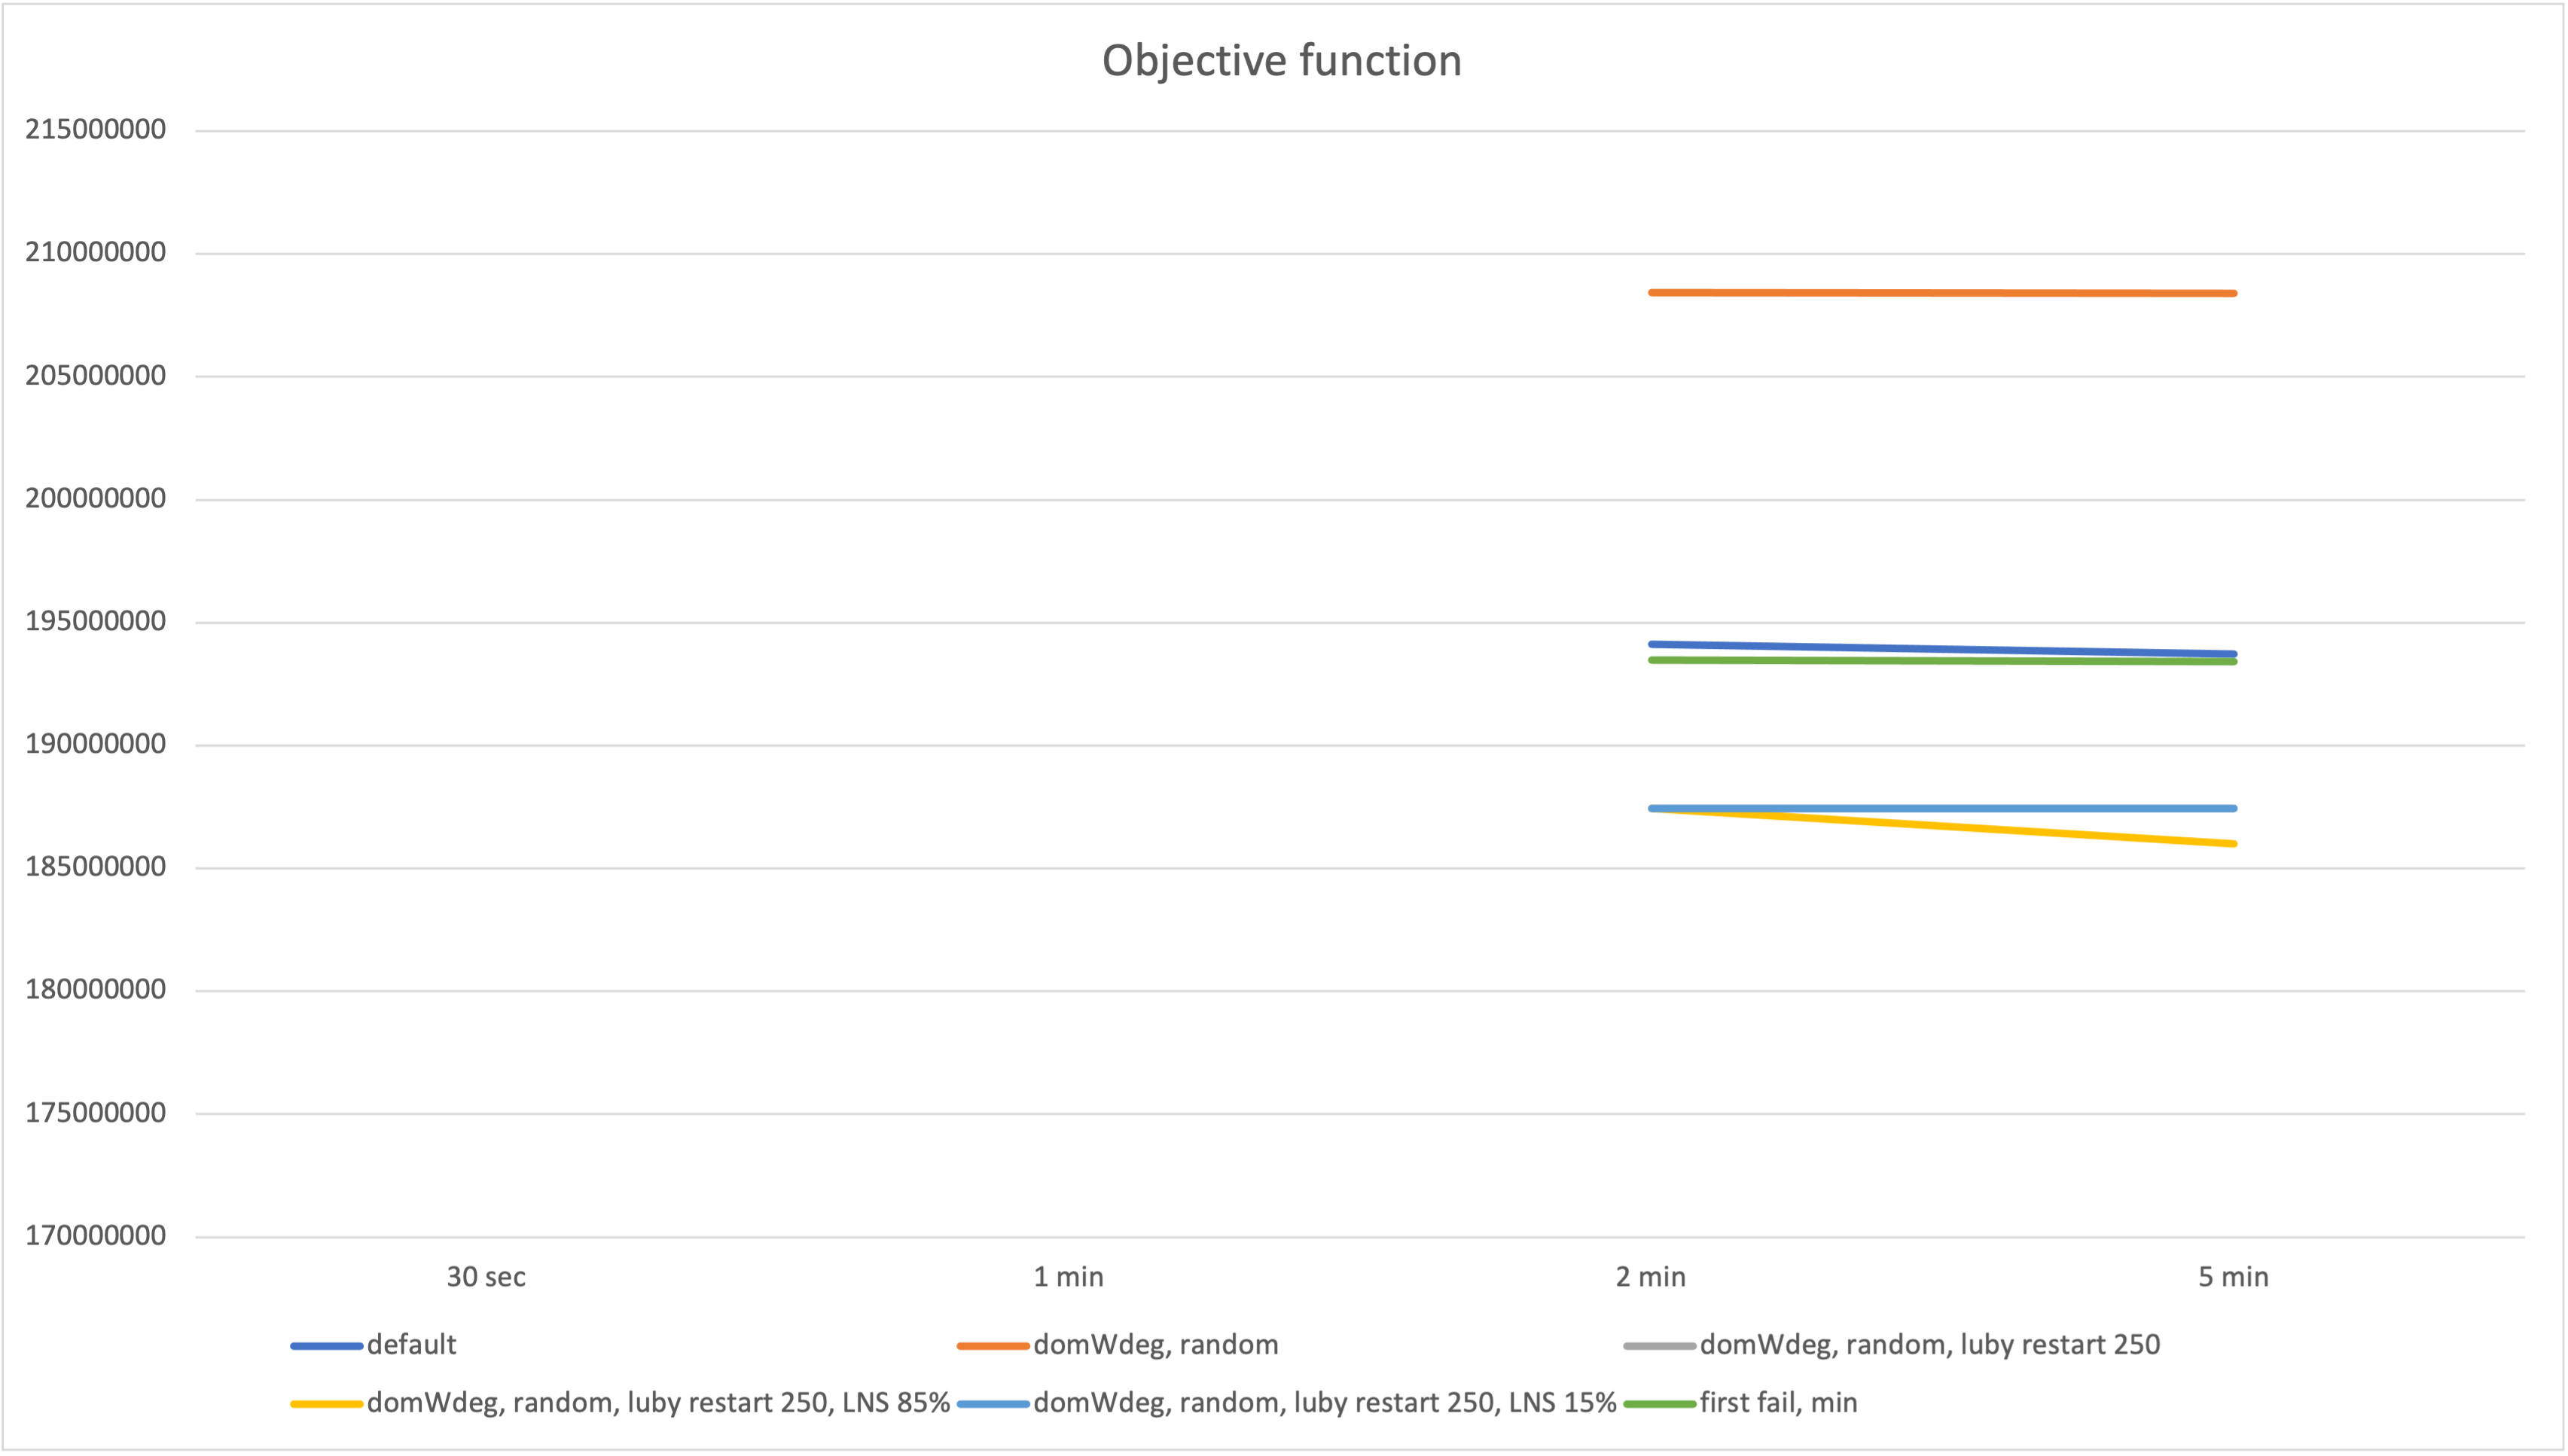
\includegraphics[width=0.8\columnwidth]{../graphs/pr06-objf.png}
    \caption{Objective functions graph for \textbf{pr06}.}
\end{figure}

{
\renewcommand{\arraystretch}{2}
\begin{longtable}[h]{| c | c | c | c |}
    \hline
    \textbf{Weights} & \textbf{Objective function} & \textbf{Total distance} & \textbf{Used vehicles} \\
    \hline
    \endhead
    $\alpha = 10, \beta = 0$ & 186.010.030 & 18.601.003 & 20 \\
    \hline
    $\alpha = 7, \beta = 3$  & 130.207.081 & 18.601.003 & 20 \\
    \hline
    $\alpha = 5, \beta = 5$  &  93.005.115 & 18.601.003 & 20 \\
    \hline
    $\alpha = 3, \beta = 7$  &  55.803.149 & 18.601.003 & 20 \\
    \hline
    $\alpha = 0, \beta = 10$ &         200 & 18.744.002 & 20 \\
    \hline
\end{longtable}
}
\begin{figure}[H]
    \centering
    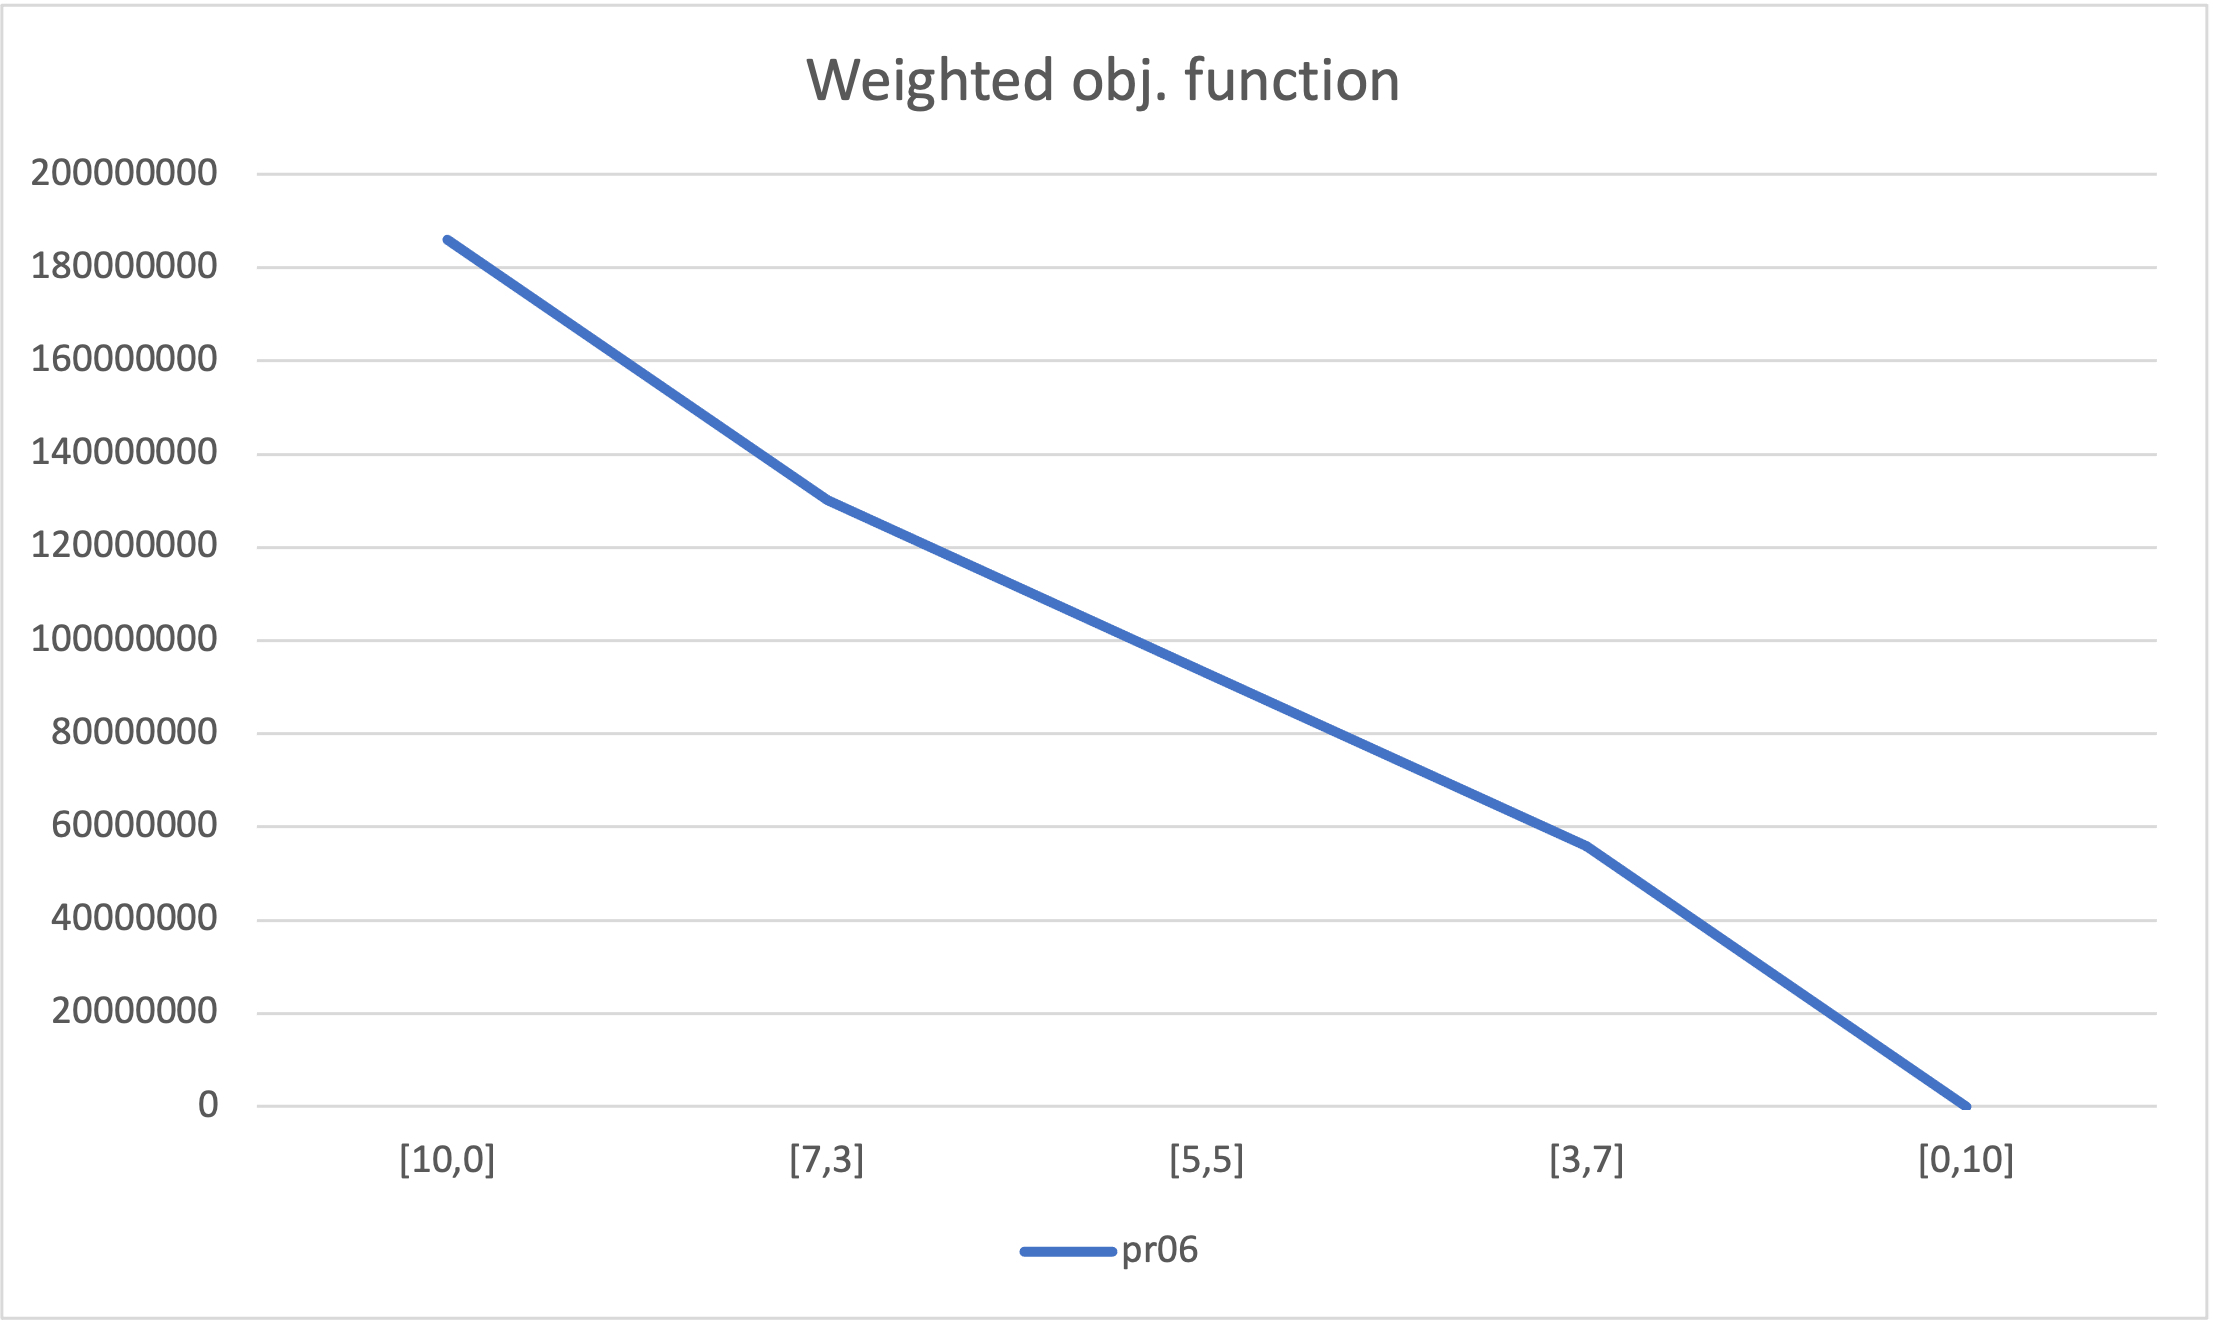
\includegraphics[height=0.25\textheight]{../graphs/pr06-wobjf.png}
    \caption{Weighted objective functions graph for \textbf{pr06}.}
\end{figure}

\begin{figure}[H]
    \centering
    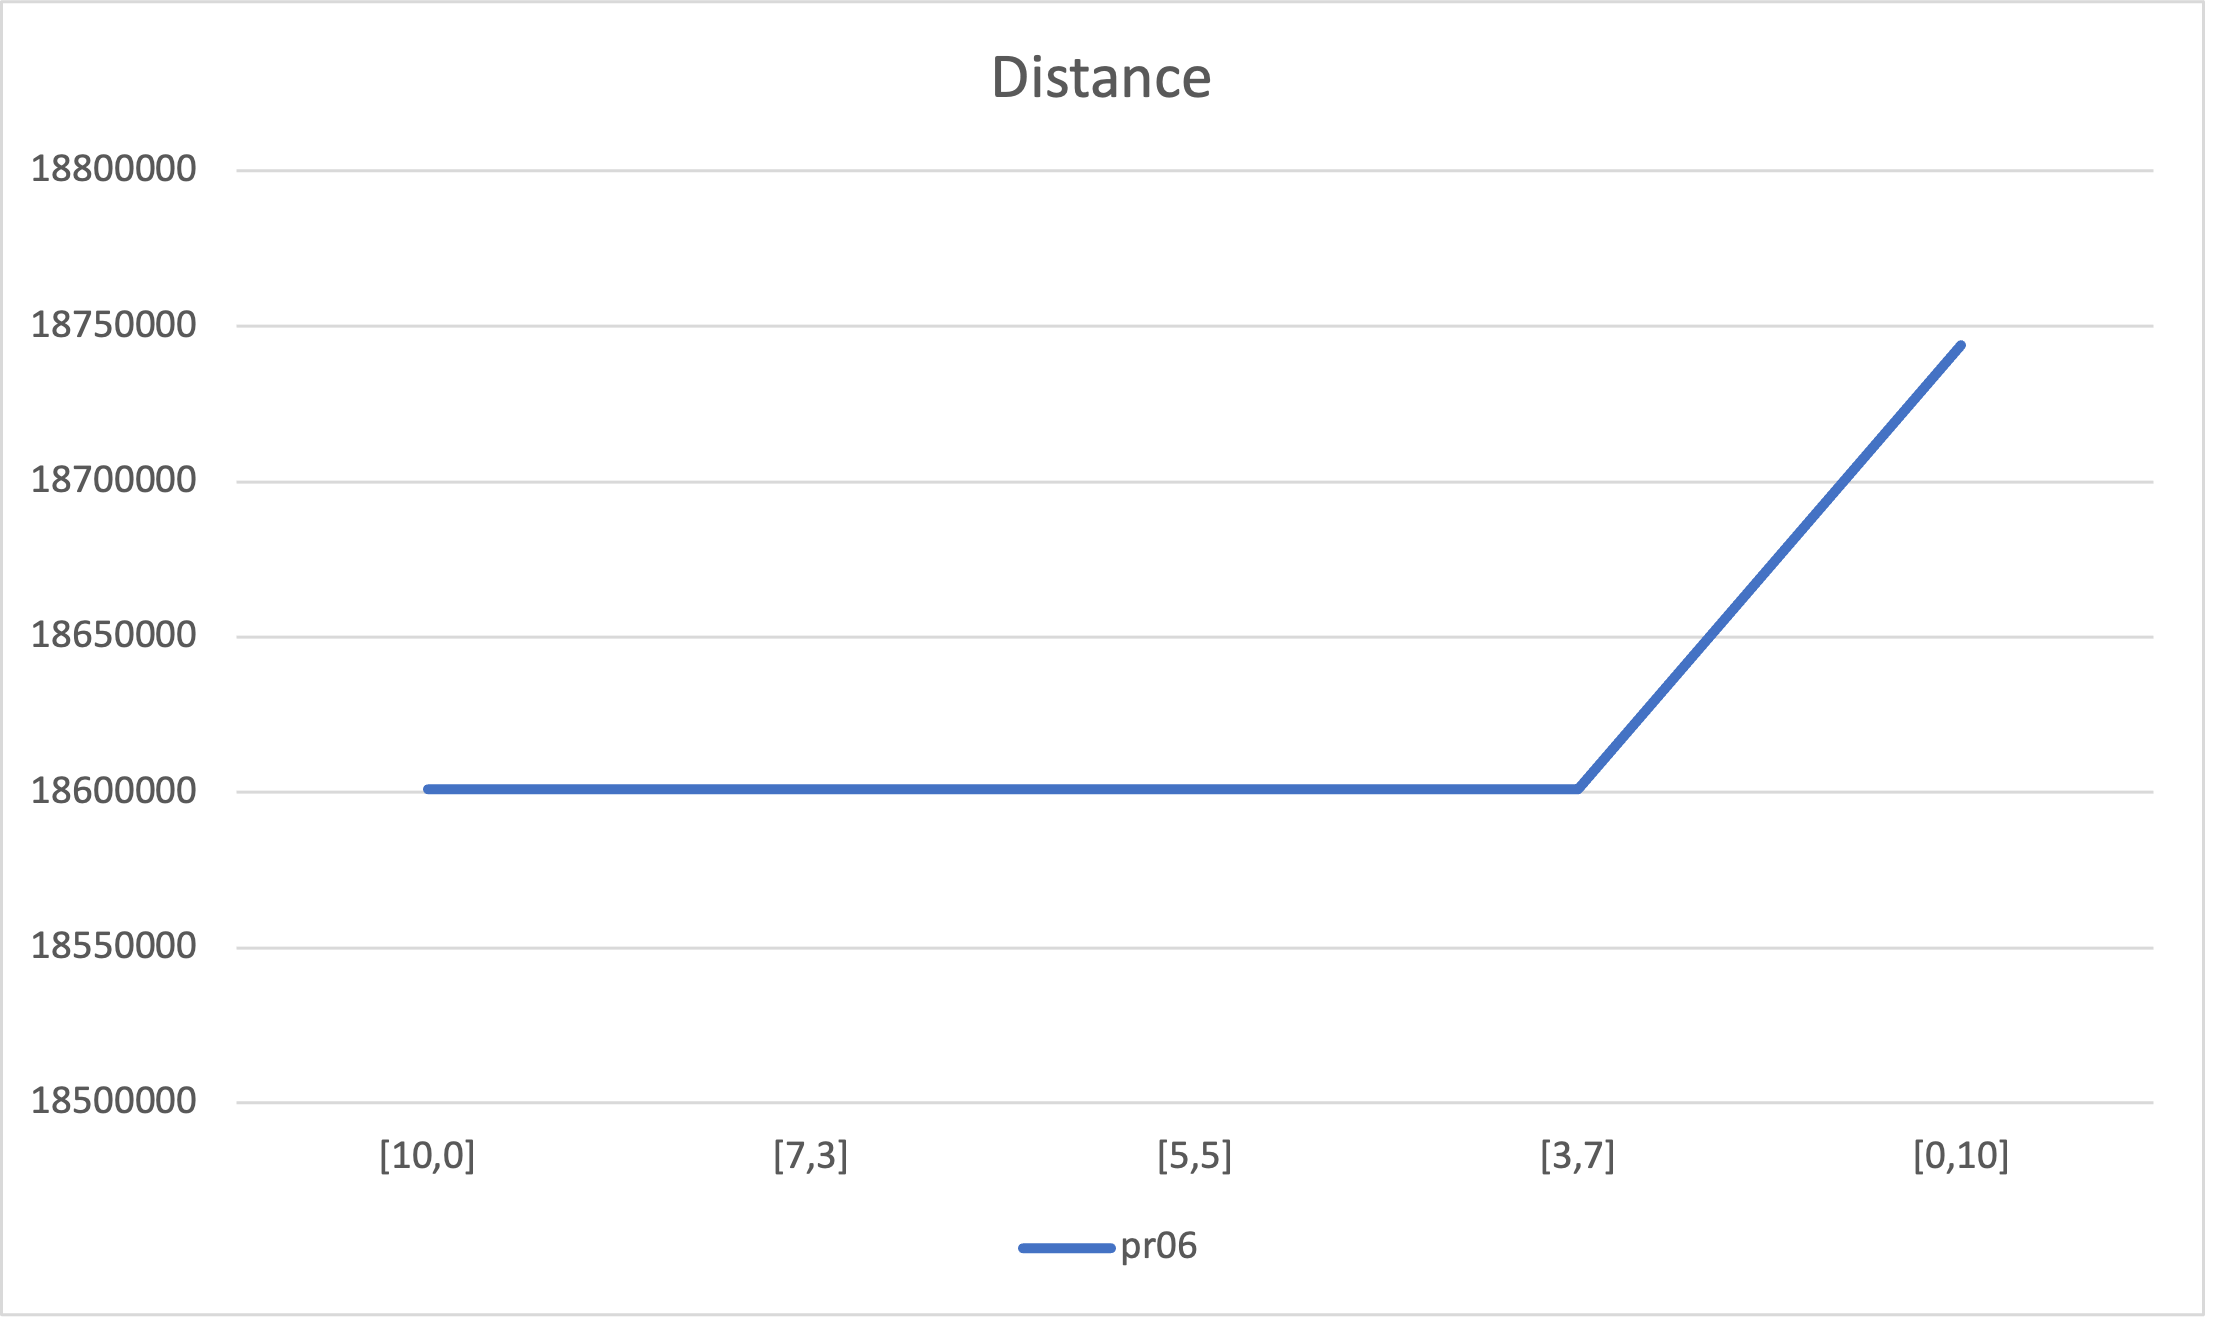
\includegraphics[height=0.25\textheight]{../graphs/pr06-distance.png}
    \caption{Distances graph for \textbf{pr06}.}
\end{figure}

\begin{figure}[H]
    \centering
    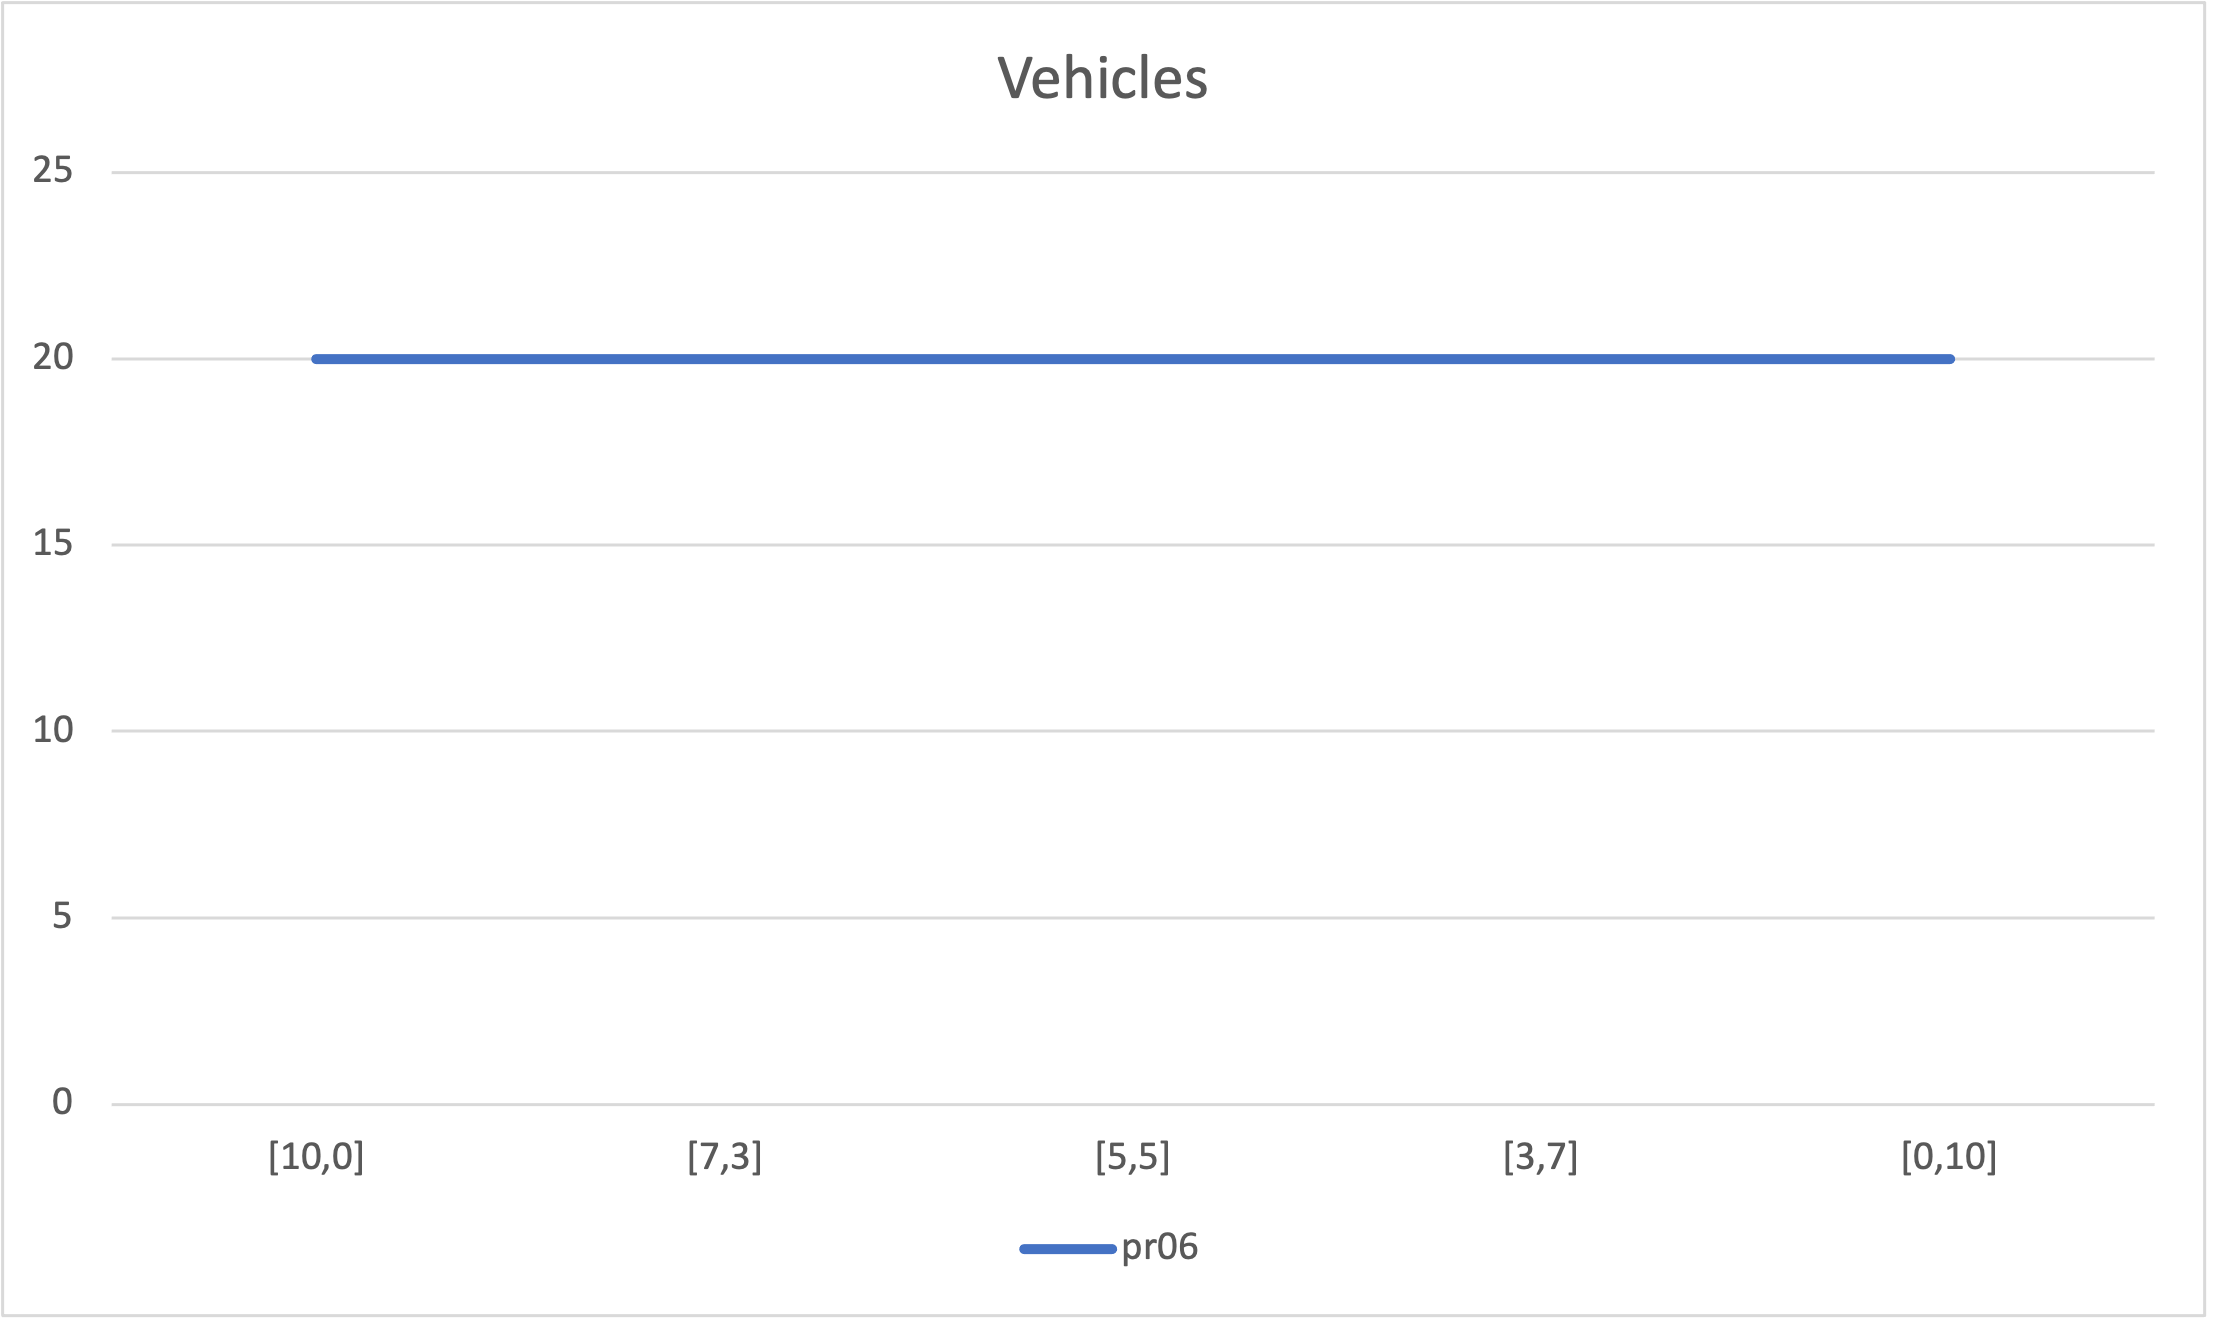
\includegraphics[height=0.25\textheight]{../graphs/pr06-vehicles.png}
    \caption{Vehicles used graph for \textbf{pr06}.}
\end{figure}

\newpage
